\documentclass[conference]{IEEEtran}
\IEEEoverridecommandlockouts
\usepackage[T1]{fontenc}
\usepackage{cite}
\usepackage{amsmath,amssymb}
\usepackage{graphicx}
\usepackage{booktabs}
\usepackage{multirow}
\usepackage{xcolor}
\usepackage{algorithm}
\usepackage{algpseudocode}
\usepackage{url}
\def\BibTeX{{\rm B\kern-.05em{\sc i\kern-.025em b}\kern-.08em
    T\kern-.1667em\lower.7ex\hbox{E}\kern-.125emX}}

\begin{document}

\title{Repeatability-Calibrated EMG--Kinematic Discordance in Pediatric Gait: A Cross-Sectional and Longitudinal Pilot Study with Wearable Sensors}

\author{
\IEEEauthorblockN{Deepinder Singh}
\IEEEauthorblockA{
\textit{Amity School of Engineering and Technology}\\
\textit{Amity University Punjab}\\
Mohali, India\\
deepinders0627@gmail.com\\
ORCID: \textcolor{red}{0000-0000-0000-0000} % TODO: replace with your ORCID iD
}
\and
\IEEEauthorblockN{Vishwanath Bijalwan\IEEEauthorrefmark{1}}
\IEEEauthorblockA{
\textit{Amity School of Engineering and Technology}\\
\textit{Amity University Punjab}\\
Mohali, India\\
vishwanath.bijalwan@gmail.com\\
ORCID: \textcolor{red}{0000-0000-0000-0000} % TODO: replace with supervisor's ORCID iD
}
\and
\IEEEauthorblockN{Vijay Bhaskar Semwal}
\IEEEauthorblockA{
\textit{Maulana Azad National Institute of Technology}\\
Bhopal, Madhya Pradesh, India
}
\thanks{\IEEEauthorrefmark{1}Corresponding author:
Vishwanath Bijalwan (vishwanath.bijalwan@gmail.com).}
}

\maketitle

\begin{abstract}
Clinical gait assessment in children with cerebral palsy (CP) and idiopathic toe walking (ITW) often treats joint kinematics and surface electromyography (EMG) as separate outcomes, and rarely asks whether a deviation in one exceeds the ordinary trial-to-trial variability of the measurement. We propose an interpretable, phase-specific concordance analysis that scores ankle dorsiflexion/plantarflexion and area-normalised tibialis anterior and gastrocnemius envelopes against a typically developing (TD) reference, calibrates each score with a within-session two-trial repeatability threshold and a leave-one-out TD background rate, and assigns every visit-limb to one of four classes: both normal, ankle-only, EMG-only or both abnormal. Applied to the public wearable-sensor dataset LIVE-GaitNeuroKids (19 CP, 11 ITW and 25 TD children, 179 trials), ankle-only abnormality dominated in CP (53.2\% of visit-limbs versus 10.2\% in TD; difference +43.0 points, child-level permutation $p=0.001$), and the result held under one-vote-per-child weighting, age matching and removal of sensor offset (43.5\% versus 6.1\%, $p=0.003$). EMG-only abnormality was not elevated in CP, and an ITW excess driven by swing-phase gastrocnemius activity (19.0\% versus 8.2\%) did not reach significance. Under the stricter repeatability-based definition, no EMG-only cases remained in the CP or ITW groups, compared with 2.0\% of TD visit-limbs. Treatment-cycle-aware pairing yielded only seven valid pre/post children, of whom one showed robust kinematic improvement without EMG change. Under the proposed conservative threshold, area-normalised EMG shape deviations rarely exceeded within-session variability, indicating limited sensitivity for detecting treatment-related changes in this two-trial wearable setting.
\end{abstract}

\begin{IEEEkeywords}
cerebral palsy, idiopathic toe walking, surface electromyography, gait analysis, inertial sensors, measurement repeatability
\end{IEEEkeywords}

\section{Introduction}
Cerebral palsy (CP) and idiopathic toe walking (ITW) are common causes of equinus and toe-walking gait in children referred for clinical gait analysis. Treatments such as botulinum toxin injection, nerve ablation and casting aim to change both how the ankle moves and how the calf and shin muscles are activated. Kinematic outcomes are usually summarised with deviation indices such as the Gait Deviation Index and the Gait Profile Score~\cite{schwartz2008gdi,baker2009gps}, and EMG has analogous indices that measure the distance of activation envelopes from a typical reference~\cite{davoudi2025fingerprint}. These measures are, however, usually reported side by side rather than jointly, so the clinically interesting case in which the two modalities disagree is not made explicit.

Disagreement between movement and muscle activation is plausible. In a randomised trial, botulinum toxin with rehabilitation improved gait kinematics in children with CP without improving surface EMG patterns~\cite{vanderhouwen2011btx}, and in a cohort of 51 patients the relation between kinematic abnormality and abnormal activation patterns was not direct~\cite{syczewska2016emg}. Detecting such disagreement in an individual child is difficult because pediatric EMG is variable: within-session waveform variability in children is roughly twice that of adults~\cite{granata2005repeat}, and repeatability baselines are needed before a between-visit change can be called real~\cite{steele2019repeat}. A discordance flag that ignores this variability risks labelling noise as a clinical finding.

The recently released LIVE-GaitNeuroKids dataset~\cite{fernandez2026live,zenodo2026live} provides synchronised inertial kinematics and four-channel surface EMG from children with CP, ITW and TD controls, two walking trials per session and repeated clinical assessments around treatment. This makes it possible to calibrate a concordance analysis against same-day repeatability using wearable rather than laboratory instrumentation. The contributions of this paper are:
\begin{itemize}
\item a visit-level, phase-specific four-class concordance analysis of ankle kinematics and tibialis anterior/gastrocnemius EMG, calibrated by a within-session two-trial repeatability threshold and a leave-one-out TD background rate;
\item to our knowledge, the first such analysis on LIVE-GaitNeuroKids, with child-level inference, age matching and a sensor-offset sensitivity analysis;
\item evidence that area-normalised EMG shape deviations rarely exceed same-day variability, together with a treatment-cycle-aware pairing of the dataset's longitudinal visits that exposes how few valid pre/post pairs it contains.
\end{itemize}

\section{Related Work}
\textbf{Gait deviation indices.} The Gait Deviation Index and Gait Profile Score summarise kinematic distance from a TD reference~\cite{schwartz2008gdi,baker2009gps}. EMG analogues include the Kerpape-Rennes EMG-based gait index and the EMG Profile Score, the latter being a mean per-muscle root mean square error (RMSE) from TD envelopes, and synergy-based dynamic motor control indices~\cite{davoudi2025fingerprint,schwartz2016dmc}. Our per-muscle RMSE is closely related to the EMG Profile Score; the novelty here lies in the joint classification and its calibration, not in the score itself.

\textbf{EMG and kinematics after treatment.} Kinematic improvement without EMG pattern change after botulinum toxin~\cite{vanderhouwen2011btx}, an indirect relation between EMG and kinematic abnormality~\cite{syczewska2016emg}, and systematic post-surgical EMG change despite stable motor-control indices~\cite{davoudi2025fingerprint} all motivate analysing the two modalities jointly.

\textbf{Repeatability.} Within-session EMG variability in healthy children exceeds adult values~\cite{granata2005repeat}, and inter-visit EMG repeatability in CP is comparable to that of unimpaired individuals~\cite{steele2019repeat}. Standard error of measurement and minimal detectable change are the usual tools for separating real change from measurement error~\cite{weir2005icc}. We use the simplest within-session analogue that two trials allow.

\textbf{Toe walking.} Premature swing-phase gastrocnemius activity has been reported in both mild diplegic CP and ITW~\cite{policy2001itw}, and botulinum toxin can normalise ankle EMG timing in ITW~\cite{brunt2004itw}.

\section{Methodology}
\subsection{Dataset}
We used version 1.1 of the public LIVE-GaitNeuroKids dataset (Zenodo, CC BY 4.0)~\cite{fernandez2026live,zenodo2026live}. Kinematics were recorded with a lower-body inertial system at 100\,Hz and surface EMG from bilateral tibialis anterior (TA) and medial gastrocnemius (GM) placed following SENIAM~\cite{hermens2000seniam}. The providers band-pass filtered (20--400\,Hz), rectified and low-pass filtered (6\,Hz) the EMG, synchronised it with the kinematics, segmented gait cycles and resampled each to 101 samples, with per-sample support (foot contact) labels. Each session contains two walking trials over a 12\,m path. CP and ITW children were assessed immediately before treatment (T0), 1--2 weeks after (T1) and about three months after (T2). We used only these processed cycles.

The public dataset contained 59 children: 22 with CP, 12 with ITW, and 25 TD controls. Our processing pipeline successfully loaded 179 trial files from 55 children, comprising 19 CP, 11 ITW, and 25 TD participants. After excluding 19 limb records for which the corresponding ankle-angle data were unavailable, 339 trial-limb records remained. The cross-sectional concordance analysis included 153 visit-limbs, whereas the repeatability thresholds were estimated from 151 visit-limbs containing at least two valid trials. These sample sets differed because repeatability estimation required paired within-session trials and used all recorded limbs, including the unaffected limb in hemiparetic and monoparetic CP, whereas concordance classification used visit-level mean scores of the analysed limbs only; this is why the repeatability set contains more CP visit-limbs (75) than the concordance analysis (62).

\subsection{Signal preparation}
For each trial and limb we used the sagittal ankle angle and the TA and GM envelopes. Each EMG cycle $e(t)$ was divided by its area, $\tilde e(t)=101\,e(t)/\sum_t e(t)$, so that 1.0 equals the cycle-mean activation and only the shape (timing) of activation is compared. Cycles were averaged within a trial. Because the kinematic and EMG sheets could contain different numbers of cycles, the stance/swing boundary was set per trial-limb to the median first sample at which the support label switched from contact to no contact (median 52\% of the cycle, range 35--81\%). For hemiparetic and monoparetic CP only the affected limb was analysed; both limbs were analysed for diparetic CP, ITW and TD.


A mean waveform was computed for each TD child over all trials and limbs, and the reference was the unweighted mean across children, so each child contributes equally (Fig.~\ref{fig:ref}). For channel $c\in\{\text{ankle},\text{TA},\text{GM}\}$ and phase $\phi\in\{\text{stance},\text{swing}\}$ the deviation score is
\begin{equation}
d_{c,\phi}=\sqrt{\frac{1}{|\phi|}\sum_{t\in\phi}\big(x_c(t)-r_c(t)\big)^2},
\end{equation}
giving six scores per trial-limb (ankle in degrees, EMG in units of cycle-mean activation). TD children were scored against a leave-one-out reference that excludes them. Visit-limb scores are the mean over the visit's trials.

\begin{figure*}[t]
\centering
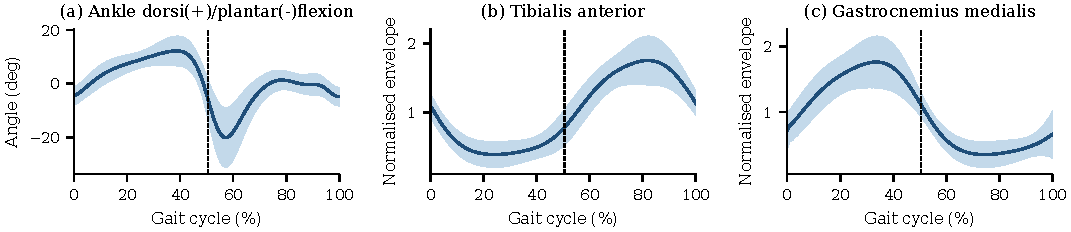
\includegraphics[width=\textwidth]{figs/fig_reference.pdf}
\caption{TD reference waveforms from 25 children (line: mean of per-child means; band: $\pm1$ SD between children; dashed line: median toe-off). EMG is area-normalised so that 1.0 is the cycle-mean activation.}
\label{fig:ref}
\end{figure*}

For every visit-limb with at least two trials (151 visit-limbs: 45 TD, 75 CP, 31 ITW), we took the absolute score difference between the first two trials. The within-session repeatability threshold $\delta_s$ for each score $s$ is the 95th percentile of these differences, pooled over groups (Table~\ref{tab:thr}). The normal limit $U_s$ is the 95th percentile of TD visit-limb scores; for a TD child it is recomputed without that child. The stricter threshold, $U_s+\delta_s$, was used as a conservative operational criterion for identifying deviations that exceeded both the TD normal limit and the observed within-session variability. It should not be interpreted as a clinically validated minimal detectable change. Rather, it provides a study-specific rule for reducing classifications that may arise from ordinary trial-to-trial variation.

\begin{table}[t]
\centering
\caption{Within-session repeatability thresholds $\delta_s$ and TD normal limits $U_s$}
\label{tab:thr}
\footnotesize
\begin{tabular}{lcccc}
\toprule
 & \multicolumn{2}{c}{$\delta_s$ (95th pct.)} & \multicolumn{2}{c}{$U_s$ (TD 95th pct.)} \\
\cmidrule(lr){2-3}\cmidrule(lr){4-5}
Score & Stance & Swing & Stance & Swing \\
\midrule
Ankle (deg) & 5.46 & 5.22 & 9.44 & 12.08 \\
TA (norm.)  & 0.72 & 0.66 & 0.59 & 0.85 \\
GM (norm.)  & 0.47 & 0.70 & 1.02 & 0.70 \\
\bottomrule
\end{tabular}
\end{table}

\subsection{Four-class concordance}
A visit-limb is ankle-abnormal if either ankle score exceeds $U_s$ and EMG-abnormal if any of the four EMG scores exceeds $U_s$. Crossing the two flags gives four classes: both normal, ankle-only, EMG-only and both abnormal. Under the stricter \emph{robust} definition a score must exceed $U_s+\delta_s$, that is, lie beyond the normal limit by more than same-day variability. Applying the same rule to TD children with leave-one-out limits gives the background rate against which patient groups are compared; because six scores are tested, this rate is expected to be well above 5\%.
\begin{algorithm}[t]
\caption{Repeatability-Calibrated EMG--Kinematic Concordance}
\label{alg:concordance}
\begin{algorithmic}[1]
\Require Trial-level deviation scores $d_{v,l,t,s}$, TD reference data
\Ensure Concordance class for each visit-limb $(v,l)$
\State Define ankle scores $\mathcal{S}_{A}=\{\text{ankle stance, ankle swing}\}$
\State Define EMG scores $\mathcal{S}_{E}=\{\text{TA stance, TA swing, GM stance, GM swing}\}$
\For{each score $s\in\mathcal{S}_{A}\cup\mathcal{S}_{E}$}
    \State $\delta_s \gets Q_{0.95}\!\left(
    \left|d_{v,l,1,s}-d_{v,l,2,s}\right|\right)$
    \Comment{repeatability threshold}
    \State $U_s \gets Q_{0.95}\!\left(\bar d_{v,l,s}^{\,\mathrm{TD}}\right)$
    \Comment{TD normal limit}
\EndFor
\For{each visit-limb $(v,l)$}
    \State $\bar d_{v,l,s}\gets \operatorname{mean}_{t}(d_{v,l,t,s})$
    \State $A\gets\mathbb{I}\!\left[
    \exists s\in\mathcal{S}_{A}:\bar d_{v,l,s}>U_s\right]$
    \State $E\gets\mathbb{I}\!\left[
    \exists s\in\mathcal{S}_{E}:\bar d_{v,l,s}>U_s\right]$
    \If{$A=0$ and $E=0$}
        \State class $\gets$ both normal
    \ElsIf{$A=1$ and $E=0$}
        \State class $\gets$ ankle-only
    \ElsIf{$A=0$ and $E=1$}
        \State class $\gets$ EMG-only
    \Else
        \State class $\gets$ both abnormal
    \EndIf
\EndFor
\State Repeat the classification using $U_s+\delta_s$ for the stricter definition.
\Statex \textbf{Note:} For TD children, the reference and $U_s$ are recomputed after excluding the evaluated child.
\end{algorithmic}
\end{algorithm}

Class proportions are reported over visit-limbs with 95\% confidence intervals from a cluster bootstrap over children (2000 resamples)~\cite{efron1993bootstrap}. Differences from TD are tested with a child-level permutation test (5000 permutations of group labels between children). Three checks follow: (i) a one-vote-per-child estimate, the mean over children of each child's class share; (ii) within TD (24 of 25 children had a recorded date of birth), Spearman correlation of age with each score; (iii) an age-matched re-analysis restricted to patient visits within the TD age range (5.0--12.2 years). In a sensitivity analysis each ankle curve and the reference were mean-centred before scoring, so a constant sensor offset cannot create an ankle deviation; all thresholds, limits and classes were recomputed.

\subsection{Longitudinal pilot}
Many children were treated more than once and the T0/T1/T2 labels restart with each treatment, so in most children the latest T2 preceded the latest T0. Using the treatment dates in the participant records, a T0 was paired with the follow-up (T2, else T1) of the same treatment cycle only when T0 fell between the previous and current treatment and the follow-up between the current and next treatment. A limb was discordant if at least one ankle score decreased by more than $\delta_s$ while no EMG score decreased by more than $\delta_s$.

\section{Results}
The TD reference reproduced the expected pattern (Fig.~\ref{fig:ref}): GM activity peaked in stance (33\% of the cycle) and was low in swing, TA was active around initial contact and peaked in swing (82\%), and peak plantarflexion occurred just after toe-off (57\%).


Table~\ref{tab:classes} and Fig.~\ref{fig:classes} give class proportions. TD visit-limbs fell outside the normal limits 20.4\% of the time, which is the background rate. In CP, ankle-only abnormality was the dominant class (53.2\%), whereas EMG-only abnormality (8.1\%) matched the TD rate. In ITW the ankle was rarely abnormal, and EMG-only abnormality was 19.0\%. Among ITW EMG-abnormal visit-limbs, 64\% were flagged by the GM swing score and 55\% by the TA stance score; in CP, 71\% were flagged by the TA stance score.

\begin{table}[t]
\centering
\caption{Concordance classes (\% of visit-limbs, 95\% child-bootstrap CI). $n$: visit-limbs/children; Std.: score exceeds $U_s$; Rob.: exceeds $U_s+\delta_s$}
\label{tab:classes}
\scriptsize
\setlength{\tabcolsep}{2.2pt}
\resizebox{\columnwidth}{!}{\begin{tabular}{llccc}
\toprule
Def. & Class & CP ($n$=62/19) & ITW ($n$=42/11) & TD ($n$=49/25) \\
\midrule
\multirow{4}{*}{Std.} & Both normal & 24.2 [9.0, 43.9] & 71.4 [58.8, 84.1] & 79.6 [66.7, 91.7] \\
 & Ankle-only & \textbf{53.2} [30.8, 71.3] & 2.4 [0.0, 7.5] & 10.2 [2.0, 20.4] \\
 & EMG-only & 8.1 [1.6, 17.3] & \textbf{19.0} [8.6, 30.0] & 8.2 [2.0, 16.0] \\
 & Both abn. & 14.5 [5.1, 26.8] & 7.1 [0.0, 20.0] & 2.0 [0.0, 6.2] \\
\midrule
\multirow{2}{*}{Rob.} & Ankle-only & 41.9 [24.1, 60.0] & 2.4 [0.0, 8.3] & 0.0 \\
 & EMG-only & 0.0 & 0.0 & 2.0 [0.0, 6.2] \\
\bottomrule
\end{tabular}}
\end{table}

\begin{figure}[t]
\centering
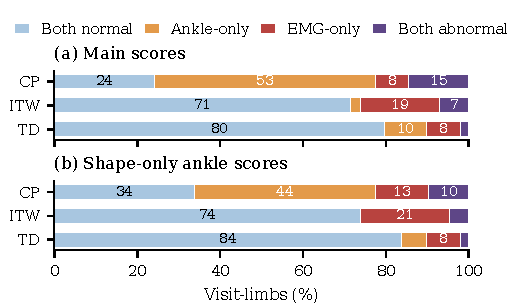
\includegraphics[width=\columnwidth]{figs/fig_classes.pdf}
\caption{Four-class concordance per group (standard definition). (a) Main scores; (b) ankle curves mean-centred to remove sensor offset. Numbers are percentages of visit-limbs.}
\label{fig:classes}
\end{figure}

Under the robust definition every EMG-only case in CP and ITW disappeared, and only CP ankle-only abnormality remained substantial (41.9\%). For most EMG scores the threshold $\delta_s$ was of the same order as, or larger than, the margin by which patient scores exceeded $U_s$ (Table~\ref{tab:thr}); for TA stance, for example, the repeatability threshold ($\delta_s=0.72$) was larger than the TD normal limit itself ($U_s=0.59$), and for GM swing the two were equal (0.70).
\begin{figure*}[htbp]
    \centering
    \includegraphics[width=0.90\textwidth]
    {Plot.png}
    \caption{Differences in concordance-class proportions between the
    clinical groups and typically developing controls. Markers represent
    the estimated differences in percentage points, and horizontal lines
    indicate 95\% child-cluster bootstrap confidence intervals. The dashed
    vertical line at zero represents no difference from the TD group.
    Positive values indicate a higher class proportion in the clinical
    group.}
    \label{fig:forest_plot}
\end{figure*}
As shown in Fig.~\ref{fig:forest_plot}, CP ankle-only abnormality was consistently higher than the corresponding TD proportion. The estimated difference was 43.0 percentage points in the main analysis ($95\%$ CI: $19.1$--$62.5$, $p=0.001$), 49.8 points in the age-range-restricted analysis ($95\%$ CI: $23.1$--$70.6$, $p<0.001$), and 37.4 points after mean-centring the ankle curves ($95\%$ CI: $14.8$--$56.9$, $p=0.003$). Because all three confidence
intervals remained above zero, the CP ankle-only finding was robust across the sensitivity analyses.

In contrast, the confidence intervals for CP EMG-only and ITW EMG-only abnormality crossed zero in every analysis. Therefore, neither group showed statistically significant evidence of an increased EMG-only proportion relative to TD controls. The positive ITW estimates suggest a possible tendency toward isolated EMG abnormality, but the available
sample does not provide sufficient evidence to confirm this difference.

Table~\ref{tab:tests} summarises the tests. Under age matching, CP ankle-only abnormality rose to 60.0\% (TD 10.2\%), and the ITW EMG-only excess was not significant in any analysis ($p=0.13$--$0.19$). One-vote-per-child estimates were close to the visit-limb rates (CP ankle-only 48.0\%, ITW EMG-only 15.9\%, TD 10.0\% and 8.0\%). Within TD, age was not associated with any score ($|\rho|\le0.20$, all $p\ge0.17$). Mean-centring the ankle curves lowered CP ankle-only abnormality to 43.5\% (TD 6.1\%) under the standard definition and to 12.9\% under the robust one, showing that part of the robust kinematic signal reflected sensor offset.
\begin{table}[t]
\centering
\caption{Difference from TD in percentage points [95\% CI] and permutation $p$. Age-matched: patient visits aged 5.0--12.2 y (CP 14/19, ITW 9/11 children)}
\label{tab:tests}
\footnotesize
\setlength{\tabcolsep}{2.5pt}
\resizebox{\columnwidth}{!}{\begin{tabular}{lccc}
\toprule
Analysis & CP ankle-only & CP EMG-only & ITW EMG-only \\
\midrule
Main & +43.0 [19.1, 62.5] & $-$0.1 [$-$10.9, 11.3] & +10.9 [$-$2.1, 23.9] \\
 & $p=0.001$ & $p=1.00$ & $p=0.18$ \\
Age-matched & +49.8 [23.1, 70.6] & $-$4.2 [$-$13.0, 5.0] & +11.3 [$-$2.6, 25.5] \\
 & $p<0.001$ & $p=0.45$ & $p=0.19$ \\
Shape-only ankle & +37.4 [14.8, 56.9] & +4.7 [$-$7.0, 18.1] & +13.3 [$-$0.5, 26.8] \\
 & $p=0.003$ & $p=0.51$ & $p=0.13$ \\
\bottomrule
\end{tabular}}
\end{table}


Only seven children had a valid same-cycle pre/post pair (three CP, four ITW; 14 limbs); two used a T2 follow-up and five a T1 follow-up (56--224 days after T0; 14--131 days after treatment). Although T1 is nominally 1--2 weeks post-treatment, T1 visits in these pairs occurred 14--98 days after treatment.A further CP child was lost because the affected limb's ankle angle was missing at T0. With the main scores, four limbs in three children were discordant (CP 2/3, ITW 1/4). After mean-centring the ankle curves only one CP child remained discordant, in both limbs (ankle stance score changes of $-$12.9 and $-$15.0 degrees). No limb showed an EMG improvement larger than $\delta_s$ under either analysis, so the pilot cannot distinguish persistent abnormal activation from changes too small to measure.

\section{Discussion}
Calibrating against same-day variability changed the picture substantially. Without it, about one visit-limb in ten in TD children and about one in four in CP (22.6\%) and ITW (26.2\%) would have been labelled EMG-abnormal. Under the stricter repeatability-based definition, no EMG-only cases remained in the CP or ITW groups, while one TD visit-limb (2.0\%) was classified as EMG-only abnormal. Area-normalised envelope shape, which captures timing but not amplitude, therefore carries limited information beyond its own measurement noise in this wearable two-trial setting. This is consistent with the high within-session variability reported for pediatric EMG~\cite{granata2005repeat} and argues for reporting repeatability alongside any EMG-based change score.

The dominant CP pattern, abnormal ankle motion with EMG shape inside the normal range, agrees with reports that kinematic abnormality in CP is not a direct consequence of abnormal activation patterns~\cite{syczewska2016emg} and that kinematics can improve after botulinum toxin without EMG pattern change~\cite{vanderhouwen2011btx}. Non-neural factors such as muscle stiffness, contracture and altered joint mechanics are plausible contributors, but our data cannot test this. The ITW trend toward swing-phase gastrocnemius activity matches the premature swing firing previously described in toe walkers~\cite{policy2001itw}, but with 11 children it remains a hypothesis.

The sensitivity analysis matters for interpretation. Removing constant ankle offset reduced robust CP ankle-only abnormality from 41.9\% to 12.9\% and the longitudinal discordance from three children to one. Inertial-sensor placement and calibration differ between sessions, and within-session repeatability does not capture this between-visit error. For treatment tracking, shape-based ankle scores or between-session repeatability data are therefore preferable.

\textit{Limitations.} The cohorts are small, especially ITW and the seven-child longitudinal pilot, and treatments were heterogeneous. Only two muscles and one joint were available. The repeatability threshold is estimated from single-trial differences while visit scores average two trials, which makes the robust definition conservative. Whole-phase RMSE can dilute brief timing errors, so an onset/offset-based timing measure might be more sensitive. One session is labelled differently in the file name and the participant records, and the detected toe-off varied widely (35--81\% of the cycle). A flag indicates measurable discordance; it does not establish treatment failure.

\section{Conclusion}
A repeatability-calibrated, phase-specific concordance analysis of wearable gait data showed that abnormal ankle kinematics with typical EMG shape characterise about half of CP visit-limbs, a result robust to child-level weighting, age matching and, under the standard definition, sensor offset. EMG shape deviations, by contrast, rarely exceeded same-day trial-to-trial variability, and the dataset contains few valid same-treatment pre/post pairs. Before EMG shape is used to track pediatric treatment response, studies should collect more trials per session, quantify between-session repeatability and test timing-specific EMG measures. The analysis code for every step is publicly available at \textcolor{red}{\url{https://github.com/deepindersinghbti/REPOSITORY-NAME}}. % TODO: replace with the final repository URL


\begin{thebibliography}{00}
\bibitem{schwartz2008gdi} M. H. Schwartz and A. Rozumalski, ``The gait deviation index: A new comprehensive index of gait pathology,'' \emph{Gait Posture}, vol. 28, no. 3, pp. 351--357, 2008.
\bibitem{baker2009gps} R. Baker \emph{et al.}, ``The gait profile score and movement analysis profile,'' \emph{Gait Posture}, vol. 30, no. 3, pp. 265--269, 2009.
\bibitem{davoudi2025fingerprint} M. Davoudi, F. Salami, R. Reisig, D. A. Patikas, N. A. Beckmann, K. S. Gather, and S. I. Wolf, ``Are electromyography data a fingerprint for patients with cerebral palsy (CP)?'' \emph{Appl. Sci.}, vol. 15, no. 2, Art. no. 766, 2025, doi: 10.3390/app15020766.
\bibitem{vanderhouwen2011btx} L. E. E. van der Houwen \emph{et al.}, ``Botulinum toxin A injections do not improve surface EMG patterns during gait in children with cerebral palsy: A randomized controlled study,'' \emph{Gait Posture}, vol. 33, no. 2, pp. 147--151, 2011.
\bibitem{syczewska2016emg} M. Syczewska and A. \'{S}wi\k{e}cicka, ``Are electromyographic patterns during gait related to abnormality level of the gait in patients with spastic cerebral palsy?'' \emph{Acta Bioeng. Biomech.}, vol. 18, no. 3, pp. 91--96, 2016, doi: 10.5277/ABB-00474-2015-02.
\bibitem{granata2005repeat} K. P. Granata, D. A. Padua, and M. F. Abel, ``Repeatability of surface EMG during gait in children,'' \emph{Gait Posture}, vol. 22, no. 4, pp. 346--350, 2005.
\bibitem{steele2019repeat} K. M. Steele, M. E. Munger, K. M. Peters, B. R. Shuman, and M. H. Schwartz, ``Repeatability of electromyography recordings and muscle synergies during gait among children with cerebral palsy,'' \emph{Gait Posture}, vol. 67, pp. 290--295, 2019.
\bibitem{fernandez2026live} C. Fern\'{a}ndez-Gonz\'{a}lez \emph{et al.}, ``LIVE-GaitNeuroKids: A multimodal and longitudinal gait dataset with inertial, video and surface electromyography in neuromotor conditions and typically developing children,'' \emph{Sci. Data}, 2026, doi: 10.1038/s41597-026-08424-4.

\bibitem{zenodo2026live} C. Fern\'{a}ndez-Gonz\'{a}lez \emph{et al.}, ``LIVE-GaitNeuroKids dataset,'' Zenodo, v1.1, 2026, doi: 10.5281/zenodo.21278362.
\bibitem{schwartz2016dmc} M. H. Schwartz, A. Rozumalski, and K. M. Steele, ``Dynamic motor control is associated with treatment outcomes for children with cerebral palsy,'' \emph{Dev. Med. Child Neurol.}, vol. 58, no. 11, pp. 1139--1145, 2016.
\bibitem{weir2005icc} J. P. Weir, ``Quantifying test-retest reliability using the intraclass correlation coefficient and the SEM,'' \emph{J. Strength Cond. Res.}, vol. 19, no. 1, pp. 231--240, 2005.
\bibitem{policy2001itw} J. F. Policy, L. Torburn, L. A. Rinsky, and J. Rose, ``Electromyographic test to differentiate mild diplegic cerebral palsy and idiopathic toe-walking,'' \emph{J. Pediatr. Orthop.}, vol. 21, no. 6, pp. 784--789, 2001.
\bibitem{brunt2004itw} D. Brunt, R. Woo, H. D. Kim, M. S. Ko, C. Senesac, and S. Li, ``Effect of botulinum toxin type A on gait of children who are idiopathic toe-walkers,'' \emph{J. Surg. Orthop. Adv.}, vol. 13, no. 3, pp. 149--155, 2004.
\bibitem{hermens2000seniam} H. J. Hermens, B. Freriks, C. Disselhorst-Klug, and G. Rau, ``Development of recommendations for SEMG sensors and sensor placement procedures,'' \emph{J. Electromyogr. Kinesiol.}, vol. 10, no. 5, pp. 361--374, 2000.
\bibitem{efron1993bootstrap} B. Efron and R. J. Tibshirani, \emph{An Introduction to the Bootstrap}. New York, NY, USA: Chapman \& Hall, 1993.
\end{thebibliography}

\end{document}
